\documentclass{article}

\usepackage[submission]{colm2026_conference}
\usepackage{booktabs}
\usepackage{graphicx}
\usepackage{microtype}
\usepackage{amsmath}
\usepackage{amssymb}
\usepackage{url}
\usepackage{hyperref}
\usepackage{pgfplots}
\usepackage{lineno}
\pgfplotsset{compat=1.18}
\definecolor{darkblue}{rgb}{0, 0, 0.5}
\hypersetup{colorlinks=true, citecolor=darkblue, linkcolor=darkblue, urlcolor=darkblue}

\title{Source and Format Matter in Process Reward Model Distillation:\\
A Controlled Diagnosis of Supervision Mismatch}

\author{Anonymous Authors}
\date{}

\begin{document}
\ifcolmsubmission
\linenumbers
\fi

\maketitle

\begin{abstract}
Process reward models (PRMs) are commonly trained from automatically generated step-level supervision, but when a small verifier fails it is often unclear whether the bottleneck is student capacity, the training recipe, or the supervision itself.
This distinction matters for efficient reasoning systems: if supervision distribution is the bottleneck, then scaling student compute or searching over nearby training recipes is wasteful until the data problem is addressed.
We study this question under a controlled setting that holds the student architecture, optimization path, and evaluation benchmark fixed while varying the source, annotation provenance, and format of process supervision.
Using the same Qwen2.5-3B score-head verifier and full ProcessBench-MATH evaluation, ProcessBench-style labels from non-MATH source splits transfer reliably to MATH: GSM8K-source supervision reaches 0.7515 mean ROC-AUC over four seeds, and OmniMath-source supervision reaches 0.7694.
OlympiadBench-source supervision is high-variance, spanning 0.5854--0.7163 over two seeds, which shows that format match alone is not sufficient.
In contrast, raw generated teacher-label supervision is markedly weaker under the same evaluation path: a 4-seed generated no-GT rank-loss baseline reaches a mean 0.6062 ROC-AUC, and a privileged-teacher-label BCE baseline reaches a mean 0.5475 ROC-AUC.
Sequence-cluster bootstrap tests over whole MATH solutions show that every GSM8K and OmniMath ProcessBench-source seed significantly beats both raw generated-label baselines.
In a same-source GSM8K control that labels the same 400 GSM8K ProcessBench candidate solutions with Gemma-4, raw generated no-GT labels reach 0.6183 mean ROC-AUC and raw generated privileged labels reach 0.5494, while GSM8K gold labels reach 0.7515.
Re-rendering those same generated labels into the ProcessBench first-error convention recovers most of the gap: no-GT rises to 0.7366 mean ROC-AUC and privileged rises to 0.6762; their 4-seed mean-score artifacts reach 0.7599 and 0.7789 ROC-AUC, respectively.
We further show that the failure is not explained by the score-head machinery alone: a matched ProcessBench-label diagnostic reaches 0.7129 ROC-AUC, while frozen-representation probes trained on generated teacher labels remain weak.
The same-source and rerender controls remove source distribution for GSM8K and identify label rendering/convention as a major failure mode, while leaving provenance and residual label-content errors coupled.
The narrower conclusion is practical: for small PRM distillation, a cheap source- and format-matched diagnostic can reveal supervision mismatch before investing in larger students or broader recipe searches.
\end{abstract}

\section{Introduction}

Process reward models assign scores to intermediate reasoning steps and are increasingly used to supervise or verify mathematical reasoning systems.
Because human step-level annotation is expensive, many PRM pipelines rely on automatically generated labels from stronger models.
This raises a practical question for efficient reasoning systems: when a distilled verifier performs poorly, should we scale the student and training budget, or should we first question whether the generated supervision matches the target evaluation distribution?
If supervision distribution is the primary bottleneck, then scaling student compute or searching over nearby training recipes is wasteful until the data problem is addressed.

We investigate this question with a controlled ablation.
We fix the verifier architecture, training path, and evaluation benchmark, and vary the source, annotation provenance, and format of step-level supervision.
The student is a Qwen2.5-3B model with a lightweight score head.
The target benchmark is full ProcessBench-MATH, evaluated over 1,000 shuffled solutions containing 6,505 reasoning steps and 594 error steps.
We compare ProcessBench-style supervision from non-MATH source splits against generated teacher labels from a privileged/no-ground-truth labeling pipeline.

The same 3B verifier that learns a transferable ProcessBench-MATH scorer from GSM8K or OmniMath ProcessBench-style labels remains weak when trained on raw generated teacher labels.
This contrast is not a state-of-the-art PRM claim: a public Qwen2.5-Math-7B-PRM800K baseline is stronger on the same split.
Instead, the contribution is diagnostic.
Under a fixed student and fixed optimizer, supervision compatibility accounts for a large difference in transfer quality, but compatibility is not binary: the high-variance OlympiadBench transfer shows that source distribution still matters even when the annotation format matches.
This suggests that some failed PRM distillation runs should be treated as data-distribution failures rather than as evidence that the student or recipe is inherently too small.

As a secondary finding, we show that teacher-level privilege does not reliably transfer into student-level verification, traceable to high symmetric label churn between privileged and non-privileged generated labels.

\paragraph{Contributions.}
First, we provide a controlled transfer diagnostic showing that ProcessBench-style GSM8K and OmniMath source labels train useful small MATH verifiers under a fixed Qwen2.5-3B score-head path, while raw generated teacher labels do not.
Second, a same-source GSM8K rerun removes source distribution as the sole explanation for the generated-label gap.
Third, a format-rerender control shows that much of the raw generated-label failure comes from label rendering/convention mismatch rather than from student capacity alone.
The resulting recommendation is data-centric: before scaling a verifier or sweeping nearby recipes, run a small source- and format-matched diagnostic to test whether the supervision distribution is compatible with the target evaluation.

\section{Experimental Setup}

\paragraph{Student and training path.}
All main trained verifiers use the same Qwen2.5-3B-Instruct backbone with a scalar score head.
We train with LoRA adapters, a score-only objective, balanced batches, binary cross-entropy for the ProcessBench-source runs, and 500 training steps.
For generated-label baselines, we report the strongest generated-label checkpoints found in our preliminary ablations and four-seed aggregate reruns for the main generated BCE/rank rows.
We also run a same-source GSM8K generated-label control: Gemma-4 labels the same 400 GSM8K ProcessBench candidate solutions used by the GSM8K gold row, with and without reference-solution access, then the student trains with the same gold-source BCE recipe.
Finally, we re-render those same generated labels into the ProcessBench first-error convention to separate raw label format from source distribution.
These generated-label baselines are not presented as a complete optimization sweep; they are included to test whether generated teacher labels can approach the same target under the same evaluation path.
The preliminary generated-label ablations span roughly ten nearby score-head training configurations, and none produces a verifier competitive with the ProcessBench-source transfers (Appendix~\ref{app:generated-ablations}).

\paragraph{Evaluation.}
All headline results evaluate on the same shuffled ProcessBench-MATH split of 1,000 solutions.
The split contains 6,505 total steps and 594 error steps.
We use exact serial scoring with batch size 1 for headline metrics, because batched score-head evaluation introduced small score perturbations that can affect ranking metrics.
We report ROC-AUC and PR-AUC as threshold-free measures.
Fixed-threshold F1 is shown only as a diagnostic, because score-head calibration varies across training conditions.

\paragraph{Label sources.}
ProcessBench-source training uses the first 400 ProcessBench examples from each source configuration, flattened into step-level labels.
The GSM8K source contains 2,082 steps, the OmniMath source contains 3,384 steps, and the OlympiadBench source contains 3,579 steps.
Exact problem-string overlap between each source file and the MATH1000 evaluation split is zero.

Generated-label training uses automatically labeled MATH-style traces from Gemma-4-26B-A4B, a publicly available mixture-of-experts teacher with roughly 26B total parameters and about 4B active parameters per token.
We distinguish labels generated with privileged access to the reference solution from labels generated without ground-truth access.
The teacher-level privilege effect is real in isolation, but the student-level transfer question is whether these generated labels yield a better answer-blind verifier.
We verified that the teacher did not simply copy ground-truth answers: only 19 of 8,008 teacher-labeled steps showed strong answer leakage (0.24\%), confirming that the teacher's labels reflect step-level judgment rather than answer copying.
For the same-source GSM8K control, the candidate solutions are the ProcessBench GSM8K source problems, matched back to GSM8K references so the privileged teacher has the same reference-solution access used in the original generated-label setup.

\paragraph{Uncertainty.}
Because multiple steps come from the same solution, the primary significance test resamples whole MATH solutions rather than individual steps.
We use a paired sequence-cluster bootstrap with 2,000 samples for the older generated-baseline ROC-AUC gaps and 5,000 samples for the same-source GSM8K and format-rerender mean-score comparisons.
These intervals quantify evaluation-sampling uncertainty for fixed checkpoints; they do not include training-seed variance for the one-seed generated-label baselines.

\section{Results}

\subsection{ProcessBench-style source labels transfer; raw generated teacher labels remain weak}

Table~\ref{tab:main} shows the main result.
With the student, training path, and evaluation held fixed, ProcessBench-style labels from GSM8K and OmniMath transfer strongly to full ProcessBench-MATH.
Raw generated teacher labels are much weaker, even when the generated-label baseline is chosen as the strongest checkpoint from the preliminary ablations.

\begin{table}[t]
\centering
\small
\resizebox{\textwidth}{!}{
\begin{tabular}{llrrrr}
\toprule
Training source & Seeds & ROC-AUC & PR-AUC & Best F1 & Fixed F1 \\
\midrule
GSM8K ProcessBench labels $\rightarrow$ MATH1000 & 0--3 & 0.7515 (0.7256--0.7760) & 0.2188 (0.1935--0.2317) & 0.3144 & 0.2503 \\
OmniMath ProcessBench labels $\rightarrow$ MATH1000 & 0--3 & 0.7694 (0.7539--0.7869) & 0.2524 (0.2277--0.2877) & 0.3276 & 0.3055 \\
OlympiadBench ProcessBench labels $\rightarrow$ MATH1000 & 0--1 & 0.6509 (0.5854--0.7163) & 0.1619 (0.1209--0.2029) & 0.2384 & 0.1938 \\
Generated privileged teacher labels, BCE & 0--3 & 0.5475 (0.5007--0.5883) & 0.0966 (0.0881--0.1045) & 0.1853 & 0.1089 \\
Generated no-GT teacher labels, rank loss & 0--3 & 0.6062 (0.5390--0.6755) & 0.1254 (0.0911--0.1672) & 0.2142 & 0.1918 \\
Same-source GSM8K generated privileged BCE & 0--3 & 0.5494 (0.4680--0.6371) & 0.0985 (0.0809--0.1235) & 0.1931 & 0.1741 \\
Same-source GSM8K generated no-GT BCE & 0--3 & 0.6183 (0.5849--0.6614) & 0.1152 (0.1049--0.1314) & 0.2168 & 0.2088 \\
Same-source GSM8K generated priv BCE, PB-format & 0--3 & 0.6762 (0.5869--0.7891) & 0.1761 (0.1175--0.2811) & 0.2554 & 0.2385 \\
Same-source GSM8K generated no-GT BCE, PB-format & 0--3 & 0.7366 (0.7011--0.7555) & 0.2478 (0.2266--0.2722) & 0.3215 & 0.3120 \\
Qwen2.5-Math-7B-PRM800K public baseline & 0 & 0.8379 & 0.3254 & 0.3991 & 0.3953 \\
\bottomrule
\end{tabular}}
\caption{Full ProcessBench-MATH transfer results on the same 1,000 MATH solutions. PB-format rows use the same Gemma-4 same-source labels re-rendered into the ProcessBench first-error convention. Parentheses show seed ranges for multi-seed rows. Best F1 is threshold-swept on the evaluation slice and is included only as a diagnostic.}
\label{tab:main}
\end{table}

\begin{figure}[t]
\centering
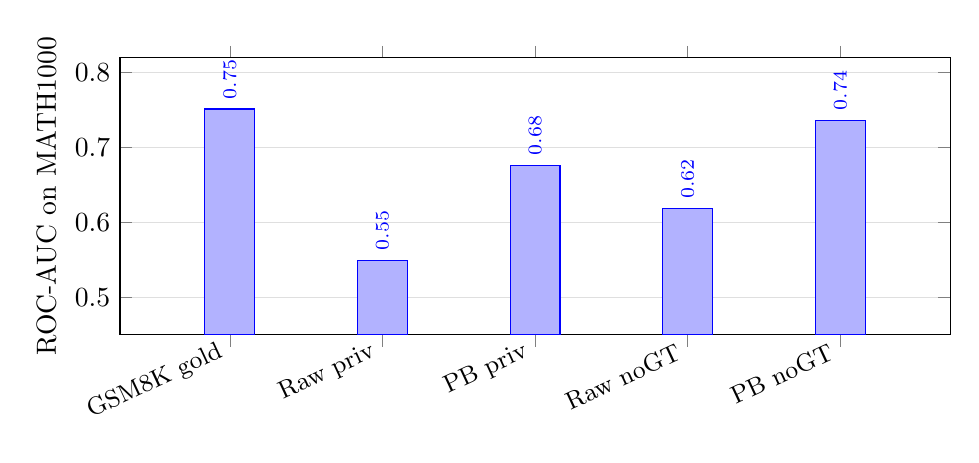
\begin{tikzpicture}
\begin{axis}[
    ybar,
    width=\textwidth,
    height=5.1cm,
    ymin=0.45,
    ymax=0.82,
    ylabel={ROC-AUC on MATH1000},
    symbolic x coords={GSM8K gold,Raw priv,PB priv,Raw noGT,PB noGT},
    xtick=data,
    x tick label style={rotate=25,anchor=east,font=\small},
    nodes near coords,
    nodes near coords style={font=\scriptsize,rotate=90,anchor=west},
    bar width=18pt,
    enlarge x limits=0.18,
    ymajorgrids=true,
    grid style={draw=gray!25},
]
\addplot coordinates {
    (GSM8K gold,0.7515)
    (Raw priv,0.5494)
    (PB priv,0.6762)
    (Raw noGT,0.6183)
    (PB noGT,0.7366)
};
\end{axis}
\end{tikzpicture}
\caption{Same-source GSM8K diagnostic: holding source problems, student, training recipe, and MATH1000 evaluation fixed, raw Gemma-4 generated labels remain far below ProcessBench gold labels; re-rendering those same labels into the ProcessBench first-error convention recovers most of the no-GT gap. This makes label convention a primary failure mode, while the remaining gap reflects residual label-content and provenance differences.}
\label{fig:main-roc}
\end{figure}

Figure~\ref{fig:main-roc} visualizes the most controlled diagnostic cell, while Table~\ref{tab:main} places it inside the broader cross-source transfer pattern.
The broader gold-vs-raw-generated contrast is large enough that it is unlikely to be an artifact of evaluation sampling.
Every GSM8K and OmniMath ProcessBench-source seed significantly beats the privileged generated-label BCE baseline under sequence-cluster bootstrap.
Against the best generated-label baseline overall, the sequence-cluster ROC-AUC gaps range from +0.0930 to +0.1546 across the eight GSM8K/OmniMath seeds, with two-sided $p=0.0010$ in all cases.
The PR-AUC gaps are proportionally larger, which is important because error steps are sparse: only 594 of 6,505 MATH evaluation steps are labeled as errors.

The public Qwen2.5-Math-7B-PRM800K checkpoint is included as an external calibration point, not as a matched training recipe.
It reaches 0.8379 ROC-AUC and remains stronger than any single 500-step ProcessBench-source seed.
This confirms that our result should not be framed as state-of-the-art PRM performance.
The central observation is instead a supervised-data compatibility mismatch: under the same small-student path, compatible ProcessBench-style supervision transfers, raw generated teacher labels do not, and convention-matched rerendering recovers much of the same-source generated-label gap.

\paragraph{Same-source GSM8K control.}
The broad gold-vs-generated contrast above changes source distribution, annotation provenance, and label semantics at once.
We therefore reran generated labeling on the same 400 GSM8K ProcessBench source problems used by the GSM8K gold row.
Holding source problems, student, optimizer, and MATH1000 evaluation fixed, raw generated labels remain far below ProcessBench gold labels: same-source generated no-GT BCE reaches 0.6183 mean ROC-AUC over four seeds and same-source generated privileged BCE reaches 0.5494, compared with 0.7515 for GSM8K gold.
Even the weakest GSM8K gold seed beats the best same-source generated no-GT seed by +0.0642 ROC-AUC under sequence-cluster bootstrap (95\% CI [0.0445, 0.0831], $p=0.0004$).
However, re-rendering those same generated labels into the ProcessBench first-error convention recovers most of the gap: the no-GT row rises to 0.7366 mean ROC-AUC and the privileged row rises to 0.6762.
Mean-score artifacts strengthen the diagnosis: PB-format no-GT and privileged 4-seed means reach 0.7599 and 0.7789 ROC-AUC, beating raw generated mean-score baselines by +0.1262 and +0.2070 under sequence-cluster bootstrap.
The PB-format privileged mean-score artifact is statistically tied with the GSM8K gold mean-score artifact (gold minus PB-format = +0.0044, 95\% CI [-0.0080, 0.0172]).
Thus source distribution is not the sole explanation, and raw label rendering/convention is a major bottleneck in this generated-label pipeline.

\subsection{Source distribution matters despite format match}

The transfer result is not a blanket claim that any non-MATH process labels transfer cleanly to MATH.
OlympiadBench is high-variance in our runs: two seeds give 0.5854 and 0.7163 ROC-AUC on full MATH1000.
One seed is significantly below the best generated-label baseline, while the other is significantly above it.
We therefore include OlympiadBench in the main table, but we do not count it as evidence for reliable transfer.
The pattern supports a source-distribution view: ProcessBench-style supervision can transfer, but matched annotation format does not by itself guarantee transfer.

\subsection{Threshold calibration agrees with the ranking result}

Fixed-threshold F1 is fragile for score-head verifiers.
To avoid choosing a threshold on the same examples used for reporting, we choose thresholds on the first 200 MATH solutions and evaluate on the remaining 800.
Under this held-out calibration protocol, GSM8K ProcessBench-source seeds reach calibrated F1 between 0.2714 and 0.3166, and OmniMath ProcessBench-source seeds reach 0.3062 to 0.3316.
OlympiadBench again splits across seeds, reaching 0.1900 and 0.2784.
The generated privileged BCE baseline reaches 0.1673, and the best generated-label baseline reaches 0.2085.
The calibrated-threshold view therefore matches the threshold-free conclusion for the reliable source splits: GSM8K and OmniMath ProcessBench-source verifiers remain well above generated-label baselines.

\section{Analysis}

\subsection{The failure is not explained by the score-head machinery alone}

A plausible concern is that the 3B score-head architecture is simply too weak to learn step-level mathematical verification.
Our diagnostics argue against that as the primary explanation.
Using the same score-head path on a matched ProcessBench-MATH split, training on the first 200 shuffled MATH examples and evaluating on the next 200 reaches 0.7129 ROC-AUC.
This is not a benchmark claim because train and evaluation data come from the same benchmark family, but it shows that the score-head machinery can learn the target when labels and distribution are aligned (Table~\ref{tab:diagnostics}).

Frozen-representation probes tell the same story.
Class-balanced logistic probes on frozen Qwen2.5-3B step-boundary embeddings trained on generated teacher labels transfer weakly to ProcessBench-MATH, around 0.52--0.56 ROC-AUC.
The corresponding matched ProcessBench-label diagnostic reaches 0.6308 ROC-AUC.
This suggests that the failure is not merely that the student representation cannot expose the target; the supervision distribution is doing meaningful work (Table~\ref{tab:diagnostics}).
The frozen-probe gap is smaller than the full score-head gap, so we treat it as a supporting diagnostic rather than a standalone explanation.

\subsection{Generated privileged labels are not reliably better student supervision}

The generated-label results also caution against a simple ``better teacher labeler implies better student'' story.
At the teacher level, privileged access to the worked reference solution improves error detection on MATH.
However, at the student level, the privileged labels do not yield a robust verifier advantage.
We do not use downstream Best-of-N reranking as evidence in this submission because an earlier symbolic-answer grading path fell back when \texttt{math\_verify} was unavailable; those downstream numbers should be regenerated before being quoted.
The evidence here is therefore limited to step-level ProcessBench metrics under corrected serial scoring.
The paired bootstrap on step-level ROC-AUC gives a priv-minus-noGT gap of -0.0098, with a 95\% confidence interval of [-0.0252, 0.0053].
We do not interpret the privileged and no-ground-truth rows in Table~\ref{tab:main} as an isolated privilege comparison, because they use different score losses.
At fixed generated-label objectives, the sign varies across ablations (Table~\ref{tab:ablations}); the safe conclusion is that we find no robust privileged-student advantage in this pipeline.

To understand why privileged teacher labels do not yield better student supervision, we examined label-level agreement.
Privileged and no-ground-truth labels agree on only 69.1\% of steps, indicating that privilege does change the training signal.
However, the disagreements are nearly symmetric: neither condition systematically corrects the other's errors.
This symmetric churn means the privileged signal does not provide a consistent directional gradient for the student to learn from.
In other words, privileged information helps the teacher perform inference-time verification, but the resulting label changes are diffuse rather than corrective.

\subsection{Training-recipe changes did not rescue generated labels}

We also tested several score-head and distillation variants before reframing the result as a supervision mismatch (Table~\ref{tab:ablations}).
Naive score-plus-critique distillation was unstable until a feedback-token truncation bug was fixed; after the fix, equal-weight critique distillation remained weak or negative for privileged labels.
Soft BCE was mostly vacuous because teacher scores were almost always binary.
Pure ranking loss and BCE-plus-rank did not rescue privileged transfer; they often favored the no-ground-truth labels.
Longer BCE training increased variance and did not turn the generated privileged labels into a competent MATH verifier.
These negative ablations do not prove that no generated-label method can work, but they reduce the likelihood that the observed gap is just a single bad optimizer setting.

\section{Related Work}

\paragraph{Process reward models for mathematical reasoning.}
PRMs have been used to provide step-level supervision and test-time verification for mathematical reasoning systems.
Math-Shepherd studies automatic process supervision for mathematical reasoning~\cite{mathshepherd}, while Qwen2.5-Math PRMs provide strong public baselines trained at much larger scale~\cite{qwenprm}.
ProcessBench evaluates earliest-error identification across multiple math reasoning sources and highlights generalization failures of existing reward models~\cite{processbench}.

\paragraph{Weak and generated process supervision.}
Recent weak-supervision approaches attempt to train PRMs without dense human process labels, using outcome labels, generated rationales, or model-derived signals~\cite{freeprm}.
These methods make PRM training more scalable, but they also raise the question studied here: when generated labels fail, is the problem the student, the recipe, or the supervision distribution?
Our experiment is complementary: rather than proposing a new weak-supervision method, we hold the small-student path fixed and compare compatible ProcessBench-style process labels against generated teacher labels.
Noise-aware PRM training directly attacks noisy process supervision through label correction and iterative denoising~\cite{noiseawareprm}.
Our controlled comparison is complementary: it first asks whether the generated-label distribution supports the target verifier under the right convention, then separates raw rendering mismatch from residual label noise.

\paragraph{Privileged on-policy distillation.}
Recent on-policy self-distillation methods condition a teacher policy on privileged solution information and distill dense token-level guidance into the same model's policy on its own rollouts~\cite{opsd,pwopsd}.
This is a different regime from ours.
We distill off-policy step-error labels from an external teacher into a separate answer-blind verifier, not token-level policy targets into the model that generated the trajectory.
Our privileged-label results therefore should not be read as contradicting successful privileged on-policy distillation; rather, they identify a failure mode for off-policy, format-sensitive verifier supervision.

\paragraph{Cross-source and out-of-distribution PRM behavior.}
Recent and concurrent work studies PRM transfer across GSM8K, MATH, OlympiadBench, OmniMath, and related sources~\cite{processlid,retrievalprm}.
Those studies motivate our source-distribution framing.
Our contribution is the controlled contrast between generated teacher labels and ProcessBench-style source labels under the same student, optimizer, and evaluation path.

\paragraph{Data-centric learning and privileged information.}
Data-centric AI work argues that systematic changes in data quality can dominate model-side changes~\cite{dataperf}.
Our result is a PRM-specific instance of that pattern: a fixed small verifier changes substantially with the supervision source.
The privileged-label experiments are also related to learning using privileged information~\cite{lupi}, but with an important boundary: privileged information can improve the teacher's per-example inference without producing labels that distill into a better answer-blind student.

\section{Limitations}

This study is diagnostic rather than prescriptive.
We evaluate one main student architecture and score-head training path, so a different student family or a substantially different distillation objective may narrow the gap.
The main comparison varies human curation, source distribution, and label format together.
The same-source GSM8K control removes source distribution for one source split, and the format-rerender cell shows that rendering/convention explains much of the raw generated-label gap.
It still does not fully isolate annotation provenance from label-content quality: the rerendered teacher first-error position disagrees with gold on roughly a quarter of source solutions.
The generated-label baselines are the strongest checkpoints from our preliminary ablations, but they are not an exhaustive search over all possible teacher prompting and label-format choices.
We therefore cannot rule out that a substantially different generated-label prompt or denoising method would further narrow the remaining gap, although the breadth of the preliminary ablations and the same-source rerun make a pure unlucky-seed explanation less likely.
The ProcessBench-source labels share the evaluation benchmark's annotation format, so part of their advantage may come from format compatibility with the evaluation benchmark.
Finally, while the public Qwen2.5-Math-7B-PRM800K baseline anchors the scale of the result, we do not compare against every recent PRM baseline under the same data budget.
The efficiency claim is also diagnostic rather than a downstream deployment claim: we defer Best-of-N reranking claims until corrected symbolic-answer grading is complete.
Instead, the practical claim is that a small source- and format-matched diagnostic can reveal whether the supervision distribution is likely to support the target verifier before larger student or recipe sweeps.

\section{Conclusion}

Under a fixed 3B verifier, training path, and ProcessBench-MATH evaluation, compatible ProcessBench-style supervision transfers much better than the generated teacher labels tested here.
The result reframes a failed privileged-feedback distillation attempt as a supervision-source, format, and distribution diagnosis.
For efficient PRM development, this suggests a practical ordering: before scaling students or re-running the same distillation loop, test whether the supervision distribution itself can support the target verifier.
In our setup, one 500-step LoRA diagnostic required approximately 0.3 GPU-hours on a single GPU, whereas the preliminary generated-label recipe sweep used approximately 15 GPU-hours across 50 runs.
This makes the diagnostic useful as an early gate before broader recipe or student-scaling sweeps.
A practical takeaway is to first run a small diagnostic with source- and format-matched labels before investing in a larger student or a new training recipe.

\section*{References}

\begin{thebibliography}{9}

\bibitem[Zheng et~al.(2024)]{processbench}
Chujie Zheng, Zhenru Zhang, Beichen Zhang, Runji Lin, Keming Lu, Bowen Yu, Dayiheng Liu, Jingren Zhou, and Junyang Lin.
\newblock ProcessBench: Identifying process errors in mathematical reasoning.
\newblock arXiv:2412.06559, 2024.

\bibitem[Wang et~al.(2023)]{mathshepherd}
Peiyi Wang, Lei Li, Zhihong Shao, Runxin Xu, Damai Dai, Yifei Li, Deli Chen, Yu Wu, and Zhifang Sui.
\newblock Math-Shepherd: Verify and reinforce LLMs step-by-step without human annotations.
\newblock arXiv:2312.08935, 2023.

\bibitem[Zhang et~al.(2025)]{qwenprm}
Zhenru Zhang, Chujie Zheng, Yangzhen Wu, Beichen Zhang, Runji Lin, Bowen Yu, Dayiheng Liu, Jingren Zhou, and Junyang Lin.
\newblock The lessons of developing process reward models in mathematical reasoning.
\newblock arXiv:2501.07301, 2025.

\bibitem[Sun et~al.(2025)]{freeprm}
Lin Sun, Chuang Liu, Xiaofeng Ma, Tao Yang, Weijia Lu, and Ning Wu.
\newblock FreePRM: Training process reward models without ground truth process labels.
\newblock arXiv:2506.03570, 2025.

\bibitem[Xie et~al.(2026)]{noiseawareprm}
Bin Xie, Bingbing Xu, Xueyun Tian, Yilin Chen, and Huawei Shen.
\newblock Towards robust process reward modeling via noise-aware learning.
\newblock arXiv:2601.12748, 2026.

\bibitem[Zhao et~al.(2026)]{opsd}
Siyan Zhao, Zhihui Xie, Mengchen Liu, Jing Huang, Guan Pang, Feiyu Chen, and Aditya Grover.
\newblock Self-distilled reasoner: On-policy self-distillation for large language models.
\newblock arXiv:2601.18734, 2026.

\bibitem[Liu et~al.(2026)]{pwopsd}
Xiaogeng Liu, Xinyan Wang, Yingzi Ma, Yechao Zhang, and Chaowei Xiao.
\newblock When are teacher tokens reliable? Position-weighted on-policy self-distillation for reasoning.
\newblock arXiv:2605.21606, 2026.

\bibitem[Zhu et~al.(2025)]{retrievalprm}
Jiachen Zhu, Congmin Zheng, Jianghao Lin, Kounianhua Du, Ying Wen, Yong Yu, Jun Wang, and Weinan Zhang.
\newblock Retrieval-Augmented Process Reward Model for Generalizable Mathematical Reasoning.
\newblock arXiv:2502.14361, 2025.

\bibitem[Bai et~al.(2026)]{processlid}
Langxing Bai, Fan Yin, Jiao Sun, and Kai-Wei Chang.
\newblock ProcessLID: Step-wise internal reward in LLM reasoning.
\newblock OpenReview 5O5AlNVAbs, 2026.

\bibitem[Mazumder et~al.(2022)]{dataperf}
Mark Mazumder et al.
\newblock DataPerf: Benchmarks for data-centric AI development.
\newblock arXiv:2207.10062, 2022.

\bibitem[Vapnik and Vashist(2009)]{lupi}
Vladimir Vapnik and Akshay Vashist.
\newblock A new learning paradigm: Learning using privileged information.
\newblock \emph{Neural Networks}, 22(5--6):544--557, 2009.

\end{thebibliography}

\appendix

\section{Additional Result Details}

\subsection{Matched-distribution and frozen-probe diagnostics}

Table~\ref{tab:diagnostics} summarizes the diagnostics used to separate score-head or representation capacity from supervision mismatch.
The matched ProcessBench score-head diagnostic shows that the training path can learn the target under distribution-matched labels, while the frozen-probe results show that generated teacher labels remain weak even when the representation is held fixed.

\begin{table}[h]
\centering
\small
\begin{tabular}{llr}
\toprule
Diagnostic & Condition & ROC-AUC \\
\midrule
Score head, matched ProcessBench-MATH 200/200 & ProcessBench labels & 0.7129 \\
Frozen probe, generated teacher labels & Privileged & 0.5497 \\
Frozen probe, generated teacher labels & No-GT & 0.5559 \\
Frozen probe, matched ProcessBench labels 200/200 & ProcessBench labels & 0.6308 \\
\bottomrule
\end{tabular}
\caption{Diagnostics showing that the score-head and frozen representation can expose the target when labels are distribution-matched.}
\label{tab:diagnostics}
\end{table}

\subsection{Sequence-cluster bootstrap gaps}

Table~\ref{tab:bootstrap} reports paired ROC-AUC gaps using sequence-cluster bootstrap over whole MATH solutions.
Every GSM8K and OmniMath ProcessBench-source seed significantly beats both raw generated-label baselines.

\begin{table}[h]
\centering
\small
\resizebox{\textwidth}{!}{
\begin{tabular}{llrr}
\toprule
Model A & Model B & ROC-AUC gap & 95\% CI \\
\midrule
GSM8K seed 0 & generated privileged BCE & +0.1932 & [0.1644, 0.2208] \\
GSM8K seed 1 & generated privileged BCE & +0.2256 & [0.2010, 0.2500] \\
GSM8K seed 2 & generated privileged BCE & +0.2099 & [0.1829, 0.2347] \\
GSM8K seed 3 & generated privileged BCE & +0.1749 & [0.1494, 0.1995] \\
OmniMath seed 0 & generated privileged BCE & +0.2033 & [0.1757, 0.2316] \\
OmniMath seed 1 & generated privileged BCE & +0.2287 & [0.1997, 0.2567] \\
OmniMath seed 2 & generated privileged BCE & +0.2072 & [0.1773, 0.2362] \\
OmniMath seed 3 & generated privileged BCE & +0.2366 & [0.2090, 0.2632] \\
\midrule
GSM8K seed 0 & best generated-label baseline & +0.1113 & [0.0874, 0.1339] \\
GSM8K seed 1 & best generated-label baseline & +0.1436 & [0.1248, 0.1627] \\
GSM8K seed 2 & best generated-label baseline & +0.1279 & [0.1067, 0.1488] \\
GSM8K seed 3 & best generated-label baseline & +0.0930 & [0.0694, 0.1156] \\
OmniMath seed 0 & best generated-label baseline & +0.1214 & [0.0964, 0.1458] \\
OmniMath seed 1 & best generated-label baseline & +0.1468 & [0.1254, 0.1676] \\
OmniMath seed 2 & best generated-label baseline & +0.1253 & [0.1026, 0.1487] \\
OmniMath seed 3 & best generated-label baseline & +0.1546 & [0.1305, 0.1773] \\
\midrule
GSM8K seed 3 & best same-source generated no-GT seed & +0.0642 & [0.0445, 0.0831] \\
GSM8K seed 3 & best same-source generated privileged seed & +0.0885 & [0.0688, 0.1080] \\
Best same-source generated no-GT seed & best same-source generated privileged seed & +0.0242 & [0.0135, 0.0344] \\
\midrule
PB-format no-GT 4-seed mean & raw no-GT 4-seed mean & +0.1262 & [0.1043, 0.1476] \\
PB-format priv 4-seed mean & raw priv 4-seed mean & +0.2070 & [0.1831, 0.2305] \\
GSM8K 4-seed mean & PB-format priv 4-seed mean & +0.0044 & [-0.0080, 0.0172] \\
GSM8K 4-seed mean & PB-format no-GT 4-seed mean & +0.0232 & [0.0113, 0.0351] \\
\bottomrule
\end{tabular}}
\caption{Sequence-cluster bootstrap ROC-AUC gaps on the MATH1000 evaluation split. The older generated-baseline rows use 2,000 bootstrap samples; the same-source GSM8K and format-rerender rows use 5,000 samples.}
\label{tab:bootstrap}
\end{table}

\subsection{Held-out threshold calibration}

Table~\ref{tab:calibration} reports thresholded metrics with thresholds chosen on the first 200 MATH solutions and evaluated on the remaining 800.

\begin{table}[h]
\centering
\small
\resizebox{\textwidth}{!}{
\begin{tabular}{lrrrr}
\toprule
Model & Calibrated F1 & Eval ROC-AUC & Eval PR-AUC & Pred error rate \\
\midrule
GSM8K ProcessBench seed 0 & 0.3166 & 0.7452 & 0.2339 & 0.2488 \\
GSM8K ProcessBench seed 1 & 0.2977 & 0.7707 & 0.2152 & 0.1466 \\
GSM8K ProcessBench seed 2 & 0.2969 & 0.7517 & 0.2261 & 0.2559 \\
GSM8K ProcessBench seed 3 & 0.2714 & 0.7233 & 0.1940 & 0.3155 \\
OmniMath ProcessBench seed 0 & 0.3062 & 0.7483 & 0.2292 & 0.2742 \\
OmniMath ProcessBench seed 1 & 0.3294 & 0.7723 & 0.2606 & 0.2321 \\
OmniMath ProcessBench seed 2 & 0.3148 & 0.7529 & 0.2327 & 0.2056 \\
OmniMath ProcessBench seed 3 & 0.3316 & 0.7855 & 0.2818 & 0.1987 \\
Generated privileged BCE & 0.1673 & 0.5490 & 0.1002 & 0.3212 \\
Best generated-label baseline & 0.2085 & 0.6314 & 0.1431 & 0.1695 \\
Qwen2.5-Math-7B-PRM800K & 0.3855 & 0.8372 & 0.3242 & 0.1091 \\
\bottomrule
\end{tabular}}
\caption{Held-out threshold calibration. Thresholds are chosen on the first 200 MATH solutions and evaluated on the remaining 800.}
\label{tab:calibration}
\end{table}

\subsection{Training-budget and score-averaging diagnostics}

Longer training is mixed.
Increasing GSM8K from 500 to 1500 steps improves seeds 0 and 1 by +0.0506 and +0.0351 ROC-AUC, respectively, but hurts seed 2 by -0.0622.
A three-seed mean of the GSM8K 1500-step checkpoints reaches 0.8153 ROC-AUC and 0.3130 PR-AUC, but remains below Qwen2.5-Math-7B-PRM800K under sequence-cluster bootstrap.
OmniMath at 1500 steps is high-variance and does not replace the four-seed 500-step main table.

Score averaging is a strong post-hoc diagnostic.
Averaging the four GSM8K seeds gives 0.7832 ROC-AUC, averaging the four OmniMath seeds gives 0.7865, and averaging all eight GSM8K+OmniMath seeds gives 0.8073.
A mixed seven-member average combining three GSM8K 1500-step seeds with four OmniMath 500-step seeds reaches 0.8276 ROC-AUC and 0.3433 PR-AUC.
This is close to the public Qwen baseline by ROC-AUC, but it is an ensemble diagnostic rather than a single-model training claim.

\section{Generated-Label Ablation Details}
\label{app:generated-ablations}

The generated-label recipe space included score-plus-critique MSE, score-only training, lower learning rates, reduced language-model loss weight, BCE with error weighting, rank-only loss, BCE-plus-rank, and longer BCE training.
The best clean privileged generated-label ROC-AUC among these preliminary ablations was a short BCE run, but it remained weak and did not become a competent verifier.
Rank-only and BCE-plus-rank strongly favored no-ground-truth labels.
These failures motivated the shift from capacity scaling to the supervision-distribution analysis in the main text.

\begin{table}[h]
\centering
\small
\resizebox{\textwidth}{!}{
\begin{tabular}{lrrl}
\toprule
Generated-label recipe & Priv ROC-AUC & NoGT ROC-AUC & Note \\
\midrule
Score+critique MSE, early 3B run & 0.4582 & 0.4870 & collapsed near all-negative threshold behavior \\
Score+critique MSE, batch-size 1 & 0.5329 & 0.4857 & unstable, many skipped/non-finite examples before truncation fix \\
Score-only MSE & 0.4844 & 0.4776 & stable but weak \\
Lower learning rate & 0.4959 & 0.4697 & collapsed/weak \\
Feedback-token truncation fixed & 0.4514 & 0.5093 & stable but negative for privileged labels \\
Reduced critique LM weight & 0.4546 & 0.4933 & stable but weak \\
BCE, error weight 3 & 0.5411 & 0.4700 & best short privileged generated-label ablation, still weak \\
Rank-only, balanced batches & 0.4939 & 0.6306 & noGT wins strongly \\
BCE+rank, balanced batches & 0.5214 & 0.6140 & noGT wins strongly \\
BCE, error weight 3, longer training & 0.4782 & 0.4971 & longer BCE degrades/nulls the privileged signal \\
\bottomrule
\end{tabular}}
\caption{Preliminary generated-label ablations on the Qwen2.5-3B score-head path. These ablations are not the main result, but they show that the generated-label weakness is not limited to a single score-head recipe.}
\label{tab:ablations}
\end{table}

\section{Reproducibility and LLM-use statement}

The main ProcessBench-source verifier runs use Qwen2.5-3B-Instruct with LoRA rank 16, LoRA alpha 32, dropout 0.05, and all linear layers targeted.
The score-head runs use a score-only objective, BCE loss, balanced batches, 500 training steps, batch size 2, model learning rate $10^{-4}$, score-head learning rate $5\times 10^{-5}$, weight decay 0.01, and serial ProcessBench evaluation with batch size 1.
The source files contain the first 400 ProcessBench examples from GSM8K or OmniMath, flattened to per-step labels.
The same-source generated GSM8K runs use \texttt{data/labeled/math\_priv\_gsm8k400\_steps.jsonl} and \texttt{data/labeled/math\_nogt\_gsm8k400\_steps.jsonl}, built by labeling the 400 GSM8K ProcessBench candidate solutions with Gemma-4 under privileged and no-ground-truth prompts.
The format-rerender runs use \texttt{data/labeled/math\_priv\_gsm8k400\_pbformat\_steps.jsonl} and \texttt{data/labeled/math\_nogt\_gsm8k400\_pbformat\_steps.jsonl}, generated by re-rendering the same teacher labels into the ProcessBench first-error convention.
Generated-label student training is offline: the teacher is not loaded during student training or evaluation because the labeled JSONL files already contain the teacher scores and feedback.
The main source-transfer jobs were run as independent single-GPU jobs; downstream Best-of-N generation and scoring were treated separately from the step-level ProcessBench metrics and are not used as evidence in this submission.

LLM assistance was used for manuscript drafting, editing, and formatting.
All reported numerical results come from experiment logs and result JSON files produced by the evaluation scripts; no reported metric was generated by an LLM.

\end{document}
